\documentclass[../../Main.tex]{subfiles}

\begin{document}
    \begin{figure}[hbt!]
        \centerline{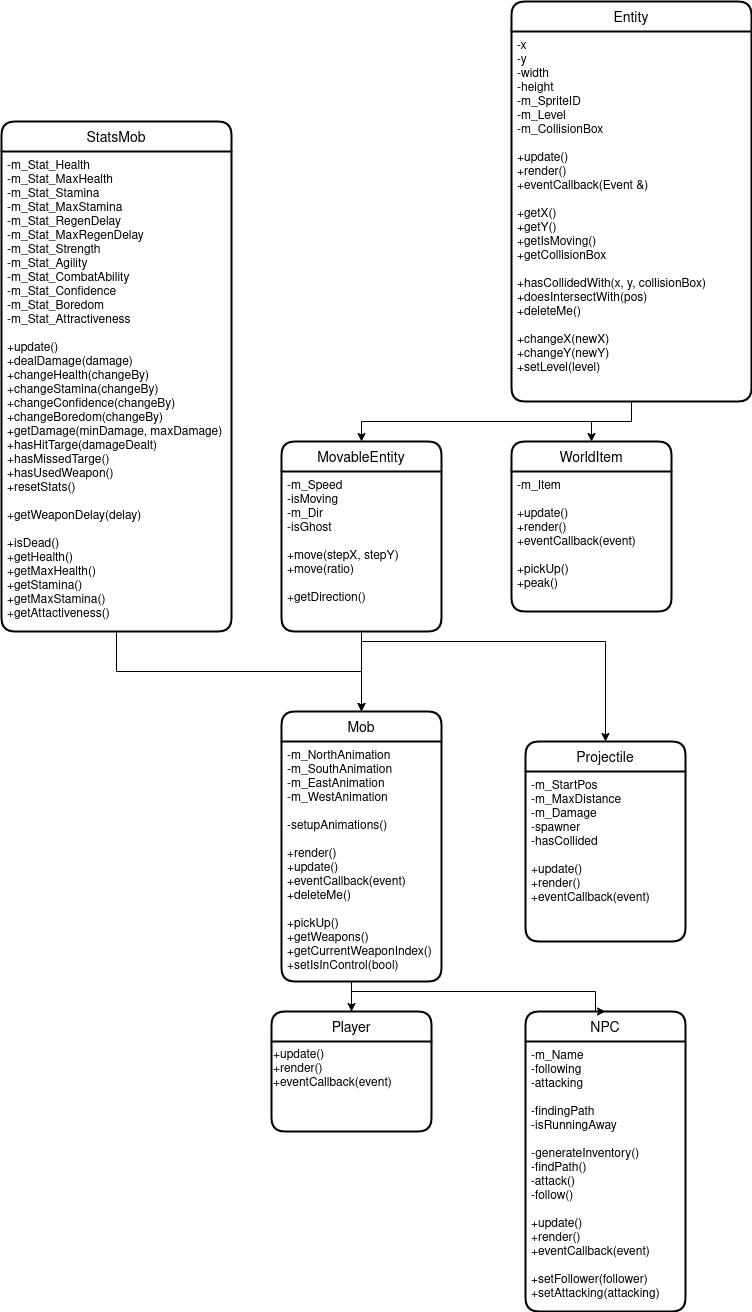
\includegraphics[scale=0.5]{img/Classes/Entities.png}}
        \caption{Entity subclasses and StatsMob}
        \label{fig}
    \end{figure}
    Entity
    \begin{center}
        Variables
        \begin{tabular}{ | m{0.45\textwidth} | m{0.45\textwidth} | }
            \hline
            \textbf{Variable Name} & \textbf{Description} \\
            \hline
            x & Stores the x position of the entity \\
            \hline
            y & Stores the y position of the entity \\
            \hline
            width & Stores the width of the entity \\
            \hline
            height & Stores the height of the entity \\
            \hline
            m\_SpriteID & Stores the sprite ID of the entity \\
            \hline
            m\_Level & Stores the level the entity is located in \\
            \hline
            m\_CollisionBox & Stores the collision box of the entity \\
            \hline
        \end{tabular}
        Functions
        \begin{tabular}{ | m{0.15\textwidth} | m{0.35\textwidth}| m{0.4\textwidth} | }
            \hline
            \textbf{Function Name} & \textbf{Parameters} & \textbf{Description} \\
            \hline
            update & & Updates the entity \\
            \hline
            render & & Renders the entity \\
            \hline
            eventCallback & Event & This allows entities to listen for events \\
            \hline
            getX & & Returns x position \\
            \hline
            getY & & Returns y position \\
            \hline
            getIsMoving & & Returns whether the entity is moving \\
            \hline
            getCollisionBox & & Returns the collision box \\
            \hline
            hasCollidedWith & position and collisionBox of an object & returns whether its collision box intersects with theirs \\
            \hline
            doesIntersectWith & position of point & returns whether or not that point is inside its collision box \\
            \hline
            deleteMe & & Returns whether the entity should be deleted \\
            \hline
            changeX & new x position & changes the x position of the entity \\
            \hline
            changeY & new y position & changes the y position of the entity \\
            \hline
            setLevel & level the entity is in & changes the level the entity is currently in \\
            \hline
        \end{tabular}
    \end{center}
    WorldItem
    \begin{center}
        Variables
        \begin{tabular}{ | m{0.45\textwidth} | m{0.45\textwidth} | }
            \hline
            \textbf{Variable Name} & \textbf{Description} \\
            \hline
            m\_Item & Stores the item that it is carrying \\
            \hline
        \end{tabular}
        Functions
        \begin{tabular}{ | m{0.15\textwidth} | m{0.35\textwidth}| m{0.4\textwidth} | }
            \hline
            \textbf{Function Name} & \textbf{Parameters} & \textbf{Description} \\
            \hline
            pickUp & & returns the item and removes it from its storage \\
            \hline
            peak & & returns the item however doesn't remove it from its storage \\
            \hline
        \end{tabular}
    \end{center}
    MovableEntity
    \begin{center}
        Variables
        \begin{tabular}{ | m{0.45\textwidth} | m{0.45\textwidth} | }
            \hline
            \textbf{Variable Name} & \textbf{Description} \\
            \hline
            m\_Speed & Stores the maximum speed it can travel at \\
            \hline
            isMoving & Stores whether it is currently moving or not \\
            \hline
            m\_Dir & Stores the direction it is travelling in \\
            \hline
            isGhost & Stores whether it ignores collision \\
            \hline
        \end{tabular}
        Functions
        \begin{tabular}{ | m{0.15\textwidth} | m{0.35\textwidth}| m{0.4\textwidth} | }
            \hline
            \textbf{Function Name} & \textbf{Parameters} & \textbf{Description} \\
            \hline
            move & Can either be a change in x and y or a ratio (using its maximum speed) & This moves the object, checking for collisions and taking into account its maximum speed \\
            \hline
            getDirection & & Returns the current direction of the entity \\
            \hline
        \end{tabular}
    \end{center}
    Projectile % TODO: This is incorrect
    \begin{center}
        Variables
        \begin{tabular}{ | m{0.45\textwidth} | m{0.45\textwidth} | }
            \hline
            \textbf{Variable Name} & \textbf{Description} \\
            \hline
            m\_StartPos & Stores the start position of the projectile \\
            \hline
            m\_MaxDistance & Stores the maximum distance the projectile can travel before being deleted \\
            \hline
            m\_Damage & Stores the maximum damage the projectile can do \\
            \hline
            spawner & Stores the Mob who spawned the projectile \\
            \hline
            hasCollided & Stores whether it has collided with anything \\
            \hline
        \end{tabular}
    \end{center}
    StatsMob
    \begin{center}
        Variables
        \begin{tabular}{ | m{0.45\textwidth} | m{0.45\textwidth} | }
            \hline
            \textbf{Variable Name} & \textbf{Description} \\
            \hline
            m\_Stat\_Health & Stores the health of the mob \\
            \hline
            m\_Stat\_MaxHealth & Stores the max health of the mob \\
            \hline
            m\_Stat\_Stamina & Stores the stamina of the mob \\
            \hline
            m\_Stat\_MaxStamina & Stores the max stamina of the mob \\
            \hline
            m\_Stat\_RegenDelay & Acts as a countdown to when the mob can start to regen its stats\\
            \hline
            m\_Stat\_MaxRegenDelay & Stores the maximum value of the regen delay counter\\
            \hline
            m\_Stat\_Strength & Stores the strength of mob \\
            \hline
            m\_Stat\_Agility & Stores the agility of the mob \\
            \hline
            m\_Stat\_CombatAbility & Stores the combat ability of the mob \\
            \hline
            m\_Stat\_Confidence & Stores the confidence of the mob (out of 100) \\
            \hline
            m\_Stat\_Boredom & Stores the boredom of the mob (out of 100) \\
            \hline
            m\_Stat\_Attractiveness & Stores the amount of followers the mob can have \\
            \hline
        \end{tabular}
        Functions
        \begin{tabular}{ | m{0.15\textwidth} | m{0.35\textwidth}| m{0.4\textwidth} | }
            \hline
            \textbf{Function Name} & \textbf{Parameters} & \textbf{Description} \\
            \hline
            update & & Updates the regen delay and handles regeneration of the mob's stats \\
            \hline
            dealDamage & max damage of weapon & Deals damage to the mob, taking into account their stats \\
            \hline
            changeHealth & changeBy & Changes the health (ignoring stats) \\
            \hline
            changeStamina & changeBy & Changes the stamina \\
            \hline
            changeConfidence & changeBy & Changes the confidence \\
            \hline
            changeBoredom & changeBy & Changes the boredom \\
            \hline
            getDamage & min and max damage of a weapon & Returns the damage the weapon should do taking into account the mob's stats \\
            \hline
            hasHitTarget & damage dealt & Increases the stats based on how much damage a weapon did \\
            \hline
            hasMissedTarget & & Changes stats for missing the targe \\
            \hline
            hasUsedWeapon & & Resets the regen delay (cannot regen while attacking) \\
            \hline
            resetStats & & Resets stats \\
            \hline
            getWeaponDelay & max delay of weapon & Returns the delay on a weapon taking into account its stats \\
            \hline
            isDead & & Returns true if the health is 0 \\
            \hline
            getHealth & & Returns the Mob's health \\
            \hline
            getMaxHealth & & Returns the max health of the mob \\
            \hline
            getStamina & & Returns the stamina of the mob \\
            \hline
            getMaxStamina & & Returns the max stamina of the mob \\
            \hline
            getAttractiveness & & Returns the attractiveness of a mob \\
            \hline
        \end{tabular}
    \end{center}
    Mob
    \begin{center}
        Variables
        \begin{tabular}{ | m{0.45\textwidth} | m{0.45\textwidth} | }
            \hline
            \textbf{Variable Name} & \textbf{Description} \\
            \hline
            m\_NorthAnimation & Stores the animation sprite for walking north \\
            \hline
            m\_SouthAnimation & Stores the animation sprite for walking south \\
            \hline
            m\_EastAnimation & Stores the animation sprite for walking east \\
            \hline
            m\_WestAnimation & Stores the animation sprite for walking west \\
            \hline
            m\_Weapons & Stores all the weapons of the mob \\
            \hline
            currentWeapon & Stores the current active weapon \\
            \hline
            m\_Inventory & Stores the inventory of the mob \\
            \hline
            isInControl & States whether the mob is inControl of its actions \\
            \hline
        \end{tabular}
        Functions
        \begin{tabular}{ | m{0.2\textwidth} | m{0.3\textwidth}| m{0.4\textwidth} | }
            \hline
            \textbf{Function Name} & \textbf{Parameters} & \textbf{Description} \\
            \hline
            setupAnimations & & Initialises the animations for each direction \\
            \hline
            pickUp & Item to pick up & Adds an item into the inventory \\
            \hline
            getWeapons & & Returns the weapons \\
            \hline
            getCurrentWeaponIndex & & Returns the current weapon index \\
            \hline
            getInventory & & Returns the inventory \\
            \hline
            setIsInControl & bool & Sets isInControl \\
            \hline
        \end{tabular}
    \end{center}
    Player \\
    The player, only overrides classes its parent classes to achieve functionality \\
    NPC
    \begin{center}
        Variables
        \begin{tabular}{ | m{0.45\textwidth} | m{0.45\textwidth} | }
            \hline
            \textbf{Variable Name} & \textbf{Description} \\
            \hline
            m\_Name & Stores the name of the follower/enemy \\
            \hline
            following & Stores the entity that it is following \\
            \hline
            attacking & Stores the entity that it is attacking \\
            \hline
            findingPath & Stores whether it is currently finding a path to take \\
            \hline
            isRunningAway & Stores whether it is running away from its enemy \\
            \hline
        \end{tabular}
        Functions
        \begin{tabular}{ | m{0.15\textwidth} | m{0.35\textwidth}| m{0.4\textwidth} | }
            \hline
            \textbf{Function Name} & \textbf{Parameters} & \textbf{Description} \\
            \hline
            generateInventory & & Generates the inventory of the NPC \\
            \hline
            findPaths & & Finds the quickest route to the entity it is following \\
            \hline
            attack & & Runs algorithm for attacking \\
            \hline
            follow & & Runs algorithm for following \\
            \hline
            setFollower & follower & Sets the entity it is following \\
            \hline
            setAttacking & attacking & Sets the entity it is attacking \\
            \hline
        \end{tabular}
    \end{center}
\end{document}